% doc type
\documentclass[12pt]{article}

% set up supplemental section
\newcommand{\beginsupplement}{%
	\setcounter{table}{0}
	\renewcommand{\thetable}{S\arabic{table}}%
	\setcounter{figure}{0}
	\renewcommand{\thefigure}{S\arabic{figure}}%
}

% format page, paragraph
\usepackage[margin=1in]{geometry}
\usepackage{lineno}
\linenumbers
\usepackage{setspace}
\doublespacing
\usepackage[utf8]{inputenc}
\usepackage[hidelinks]{hyperref}
\usepackage{authblk}

% bib - uses better biblatex
\usepackage[style=apa,backend=biber]{biblatex}
\addbibresource{./Zotero_adr_dwi.bib}

% figures and tables
\usepackage{graphicx}
\graphicspath{ {./} }
\usepackage{multirow}
\usepackage[table,xcdraw]{xcolor}
\usepackage{url}
\usepackage{float}
\usepackage{longtable}

% code
\usepackage{listings,lstautogobble}
\lstset{language=R,
	basicstyle=\small\ttfamily,
	otherkeywords={0,1,2,3,4,5,6,7,8,9},
	morekeywords={TRUE,FALSE},
	deletekeywords={data,frame,length,as,character},
	autogobble=true
}
\renewcommand\lstlistingname{R Code}

% math
\usepackage{amsmath}
\usepackage{caption}
\DeclareCaptionType{equ}[R Code][]

% title page info
\title{Longitudinal study of concussion-related diffusion MRI changes in college athletes}
\date{}

\author[1,*]{Nathan M. Muncy}
\author[1]{Heather C. Bouchard}
\author[1]{Aron K. Barbey}

\affil[1]{Center for Brain, Behavior and Biology, University of Nebraska-Lincoln, Lincoln, Nebraska, USA}
\affil[*]{Corresponding author.	Email: nmuncy2@unl.edu}

% start document
\begin{document}

% title page
\maketitle
\pagebreak


% abstract page
\begin{abstract}

% TODO: Update, finalize.

Sports-related traumatic brain injuries affect 1.6-3.8 million individuals in the US each year, and diffusion weighted imaging can measure the complex timeline of resulting axolemmal changes. Such longitudinal data is difficult to model statistically, however, given the high-dimensionality, semi-parametric and interdependent scalar values, and non-linear spatial (within-tract) and temporal (across visit) properties. Proposal: hierarchical generalized additive models (HGAMs) are well-suited to fit such data with the requisite flexibility and sensitivity to investigate (a) the spatial and temporal changes of white matter tracts, and (b) how such changes relate to diagnostic assessments. Methods: we utilized MRI and IMPACT data collected from 67 college athletes (9 female, age=19.43[1.68]) at three visits: start-of-season, post-concussion, and return-to-play. Diffusion tensors were modeled via constrained spherical deconvolution and probabilistic tractography from pyAFQ yielded 100 scalar values per white matter bundle. Results: By fitting the scalar profiles with longitudinal HGAMs we detected within-tract changes as a function of visit, revealing distinct patterns of post-injury disruption and recovery. Critically, it is unlikely that such changes would have been detected with standard techniques given their linear assumptions and limited dimensionality. Further, we examined whether these evolving diffusion metrics correlated with cognitive outcomes using HGAM tensor product interaction smooths and found moderate evidence linking white matter alterations to IMPACT composite scores. Merit: HGAMs offer a powerful framework to capture the complex progression of brain injury. Our findings suggest that HGAMs enhance our understanding of the spatiotemporal dynamics of brain injury and may enable more accurate tracking of injury and recovery.

\end{abstract}

\vfill
KEYWORDS: DWI, MRI, GAM, TBI\\
\pagebreak


\section{Introduction}
\label{sec:intro}
Introduction here.

% TODO: (Heather?) Epidemilogic description of TBI in US, athletes
% TODO: mTBI sequelae description
% TODO: DWI and mTBI
% TODO: Modeling DWI, issues
% TODO: Purpose - (a) extend GAMs for longitudinal DWI, (b) tensor product interaction smooths for multi-modal analyses


\section{Methods}
\label{sec:meth}

\subsection{Participants}
\label{ssec:meth-part}
Participants were recruited from men's football and women's soccer programs at the University of Nebraska-Lincoln, which resulted in a total of 69 (9 female, age = 19.36 $\pm$1.67, range = 17-24) National Collegiate Athletic Association (NCAA) athletes. Due to the limited number of females, and the sport-sex interaction confound, we combined all participants into a single group. Institutional Review Board approval was obtained at the outset of the study, and prior to beginning experimental procedures participants completed informed consent and assent. Magnetic Resonant Imaging (MRI) and clinical assessment (ImPACT, described below) data were acquired at three sessions: enrollment at the beginning of the season (baseline, Base), within 48 hours of diagnosed concussion (post-concussion, Post), and prior to return-to-play (RTP). As scan and ImPACT (below) data were gathered separately, a number of participants did not contribute scan and/or ImPACT data across one or more of the sessions. This resulted in the following final session counts: Base = 67 MRI (9 female), 61 ImPACT (5 female), Post = 65 MRI (8 female), 48 ImPACT (3 female), and RTP = 56 MRI (7 female), 32 ImPACT (2 female).


\subsection{ImPACT}
\label{ssec:meth-imp}
Description of ImPACT.

% TODO: (Heather) Description of ImPACT collection and items.


\subsection{MRI Protocol}
\label{ssec:meth-mri}

Magnetic Resonance Imaging data were collected on a 3 Tesla Siemens MAGNETOM Skyra scanner at the Center for Brain, Behavior and Biology (University of Nebraska-Lincoln) utilizing a 32-channel coil. For each of three sessions (Base, Post, and RTP), participants contributed T1 and diffusion weighted images (T1w, DWI). T1w Multi-Echo Magnetization Prepared - RApid GRadient Echo (MEMP-RAGE) structural scans were acquired with the following parameters: TR = 2530 ms, TE = 1.69, 3.55, 5.41, and 7.27 ms, flip angle = 7$^{\circ}$, voxel size = 1 mm$^3$, FoV = 256 $\times$ 256, slices = 176 interleaved. DWI scans were acquired via TR = 3000 ms, TE = 95 ms, flip angle = 90$^{\circ}$, voxel size = 1.719 $\times$ 1.719 $\times$ 2.4 mm$^3$, 134 slices, multi-band acceleration factor = 3, directions = 128, bandwidth = 1500 Hz/Px, shells = 1 (b-value = 1000 s/mm$^2$), reference volumes = 6 (b-values = 0 s/mm$^2$; b$_0$). A set of field maps for the DWI scans were collected using the same acquisition direction (anterior-posterior; AP) and reversed (posterior-anterior; PA).


\subsection{MRI Data Processing}
\label{ssec:meth-mri-proc}
Preprocessing and modeling of the DWI data were conducted using FSL v6.0 \parencite{jenkinson2012Fsl} and PyAFQ v1.3.6 \parencite{kruper2021EvaluatingReliabilityHuman,yeatman2012TractProfilesWhite}. First, b$_0$ volumes from AP and PA field map files were extracted and combined, as were their acquisition parameters. Next, \lstinline{topup} calculated a distortion correction matrix from the AP-PA b$_0$ file. A brain mask was generated via \lstinline{bet}, and an index file was generated to describe the relationship between the DWI volumes and their acquisition parameters. Preprocessing of DWI was then conducted via \lstinline{eddy_openmp}, which generated motion- and distortion-corrected diffusion images.

Whole-brain tractography was computed from the preprocessed DWI by PyAFQ. Constrained spherical deconvolution was used to derive the fiber orientation distribution function (fODF) of each voxel, where constrained-positivity regularization = 1, minimum amplitude $\tau$ = 0.1, mean gray matter diffusivity = 0.0008, mean CSF diffusivity = 0.003, 600 fODF iterations, and spherical harmonics order = 8. Resulting fODFs of each voxel were then utilized to probabilistically generate fiber maps, using one seed per voxel for each dimension, a maximum turning angle of 30$^\circ$, step size = 0.5 mm, and a length range = 50-250 mm. The resulting fibers were parcellated into individual tracts via \textit{a priori} inclusion (waypoint) and exclusion regions of interest \parencite{wakana2007ReproducibilityQuantitativeTractography}. Resulting tracts were then compared to a fiber probability map \parencite{hua2008TractProbabilityMaps} and any fibers which traverse low-probability spaces were removed from the tract. Further, any fibers with a length 3+ standard deviations from the tract average, or 4+ standard deviations from the average path centroid, were removed as well. Lastly, each tract was then resampled into 100 equidistant nodes (according to a Mahalanobis distance metric) for which averaged diffusion values and scalars were calculated. Specifically, for each tract node we extracted averaged axial diffusivity ($\lambda_\parallel$; AD), radial diffusivity ($(\lambda_{\perp1}+\lambda_{\perp2})/2$; RD), mean diffusivity ($(\lambda_\parallel+\lambda_{\perp1}+\lambda_{\perp2})/3$; MD), and fractional anisotropy (FA).

% TODO: Cite that CSD, prob tract are better for TBI?


\subsection{GAM specification}
\label{ssec:meth-gam}
Generalized additive models (GAM) are a generalization of general linear models capable of modeling high-dimensional, semi-parametric data that contain non-linear interaction terms. Rather than fitting data with a linear (or higher-order polynomial) function, a penalized set of basis functions (i.e. splines) is used to compose a smooth that fits the data, smooths which can exist as a 2-dimensional line (X-Y relationship), a 3-dimensional membrane termed a `tensor product interaction smooth' (X-Y-Z interactions), or as a hypersurface (4+ dimensions; \cite{baayen2020IntroductionGeneralizedAdditive}). The capability of GAMs to fit complex, high-dimensional data have made them useful in fields such as ecology ([CITE]) and linguistics ([CITE]), where complex global and local interactions across terms are well-fit, and fields using MRI modeling techniques are beginning to adopt the approach ([CITE]). We recently demonstrated their applicability to modeling DWI scalar data \parencite{muncy2022GeneralAdditiveModels}, and here we extend GAMs to model high-dimensional, longitudinal, multimodal data.


% TODO: Describe GAMMs, HGAMs
% TODO: Detail various model specifications (ImPACT, LDI, LGIO_intx) across scalars. Emphasis on LDI/LGI - utilize within-subject variance across time. Emphasis on single model - within-subject variance across tract.
% TODO: Reference github


\section{Results}
\label{sec:res}

\subsection{ImPACT}
\label{ssec:res-imp}

% TODO: Composite and total symptom GAM

The relationship between session (Base, Post, RTP) and ImPACT composite metrics (verbal memory, visual memory, visual motor, impulse control, and reaction time) and total symptom scores were modeled with GAMs to test for deflections from baseline values (Figure \ref{fig:imp-gam}). GAMs are particularly useful as non-linear trends are expected in such metrics, and further, are capable of handling the semi-parametric distributions. Specifically, verbal and visual composites were converted to proportion scores and modeled with a beta distribution, visual motor and reaction time were best fit with Gaussian distributions (despite the skewness), and impulse control and total symptoms were best fit with a negative binomial distribution.

\begin{figure}[H]
	\centering
	\fbox{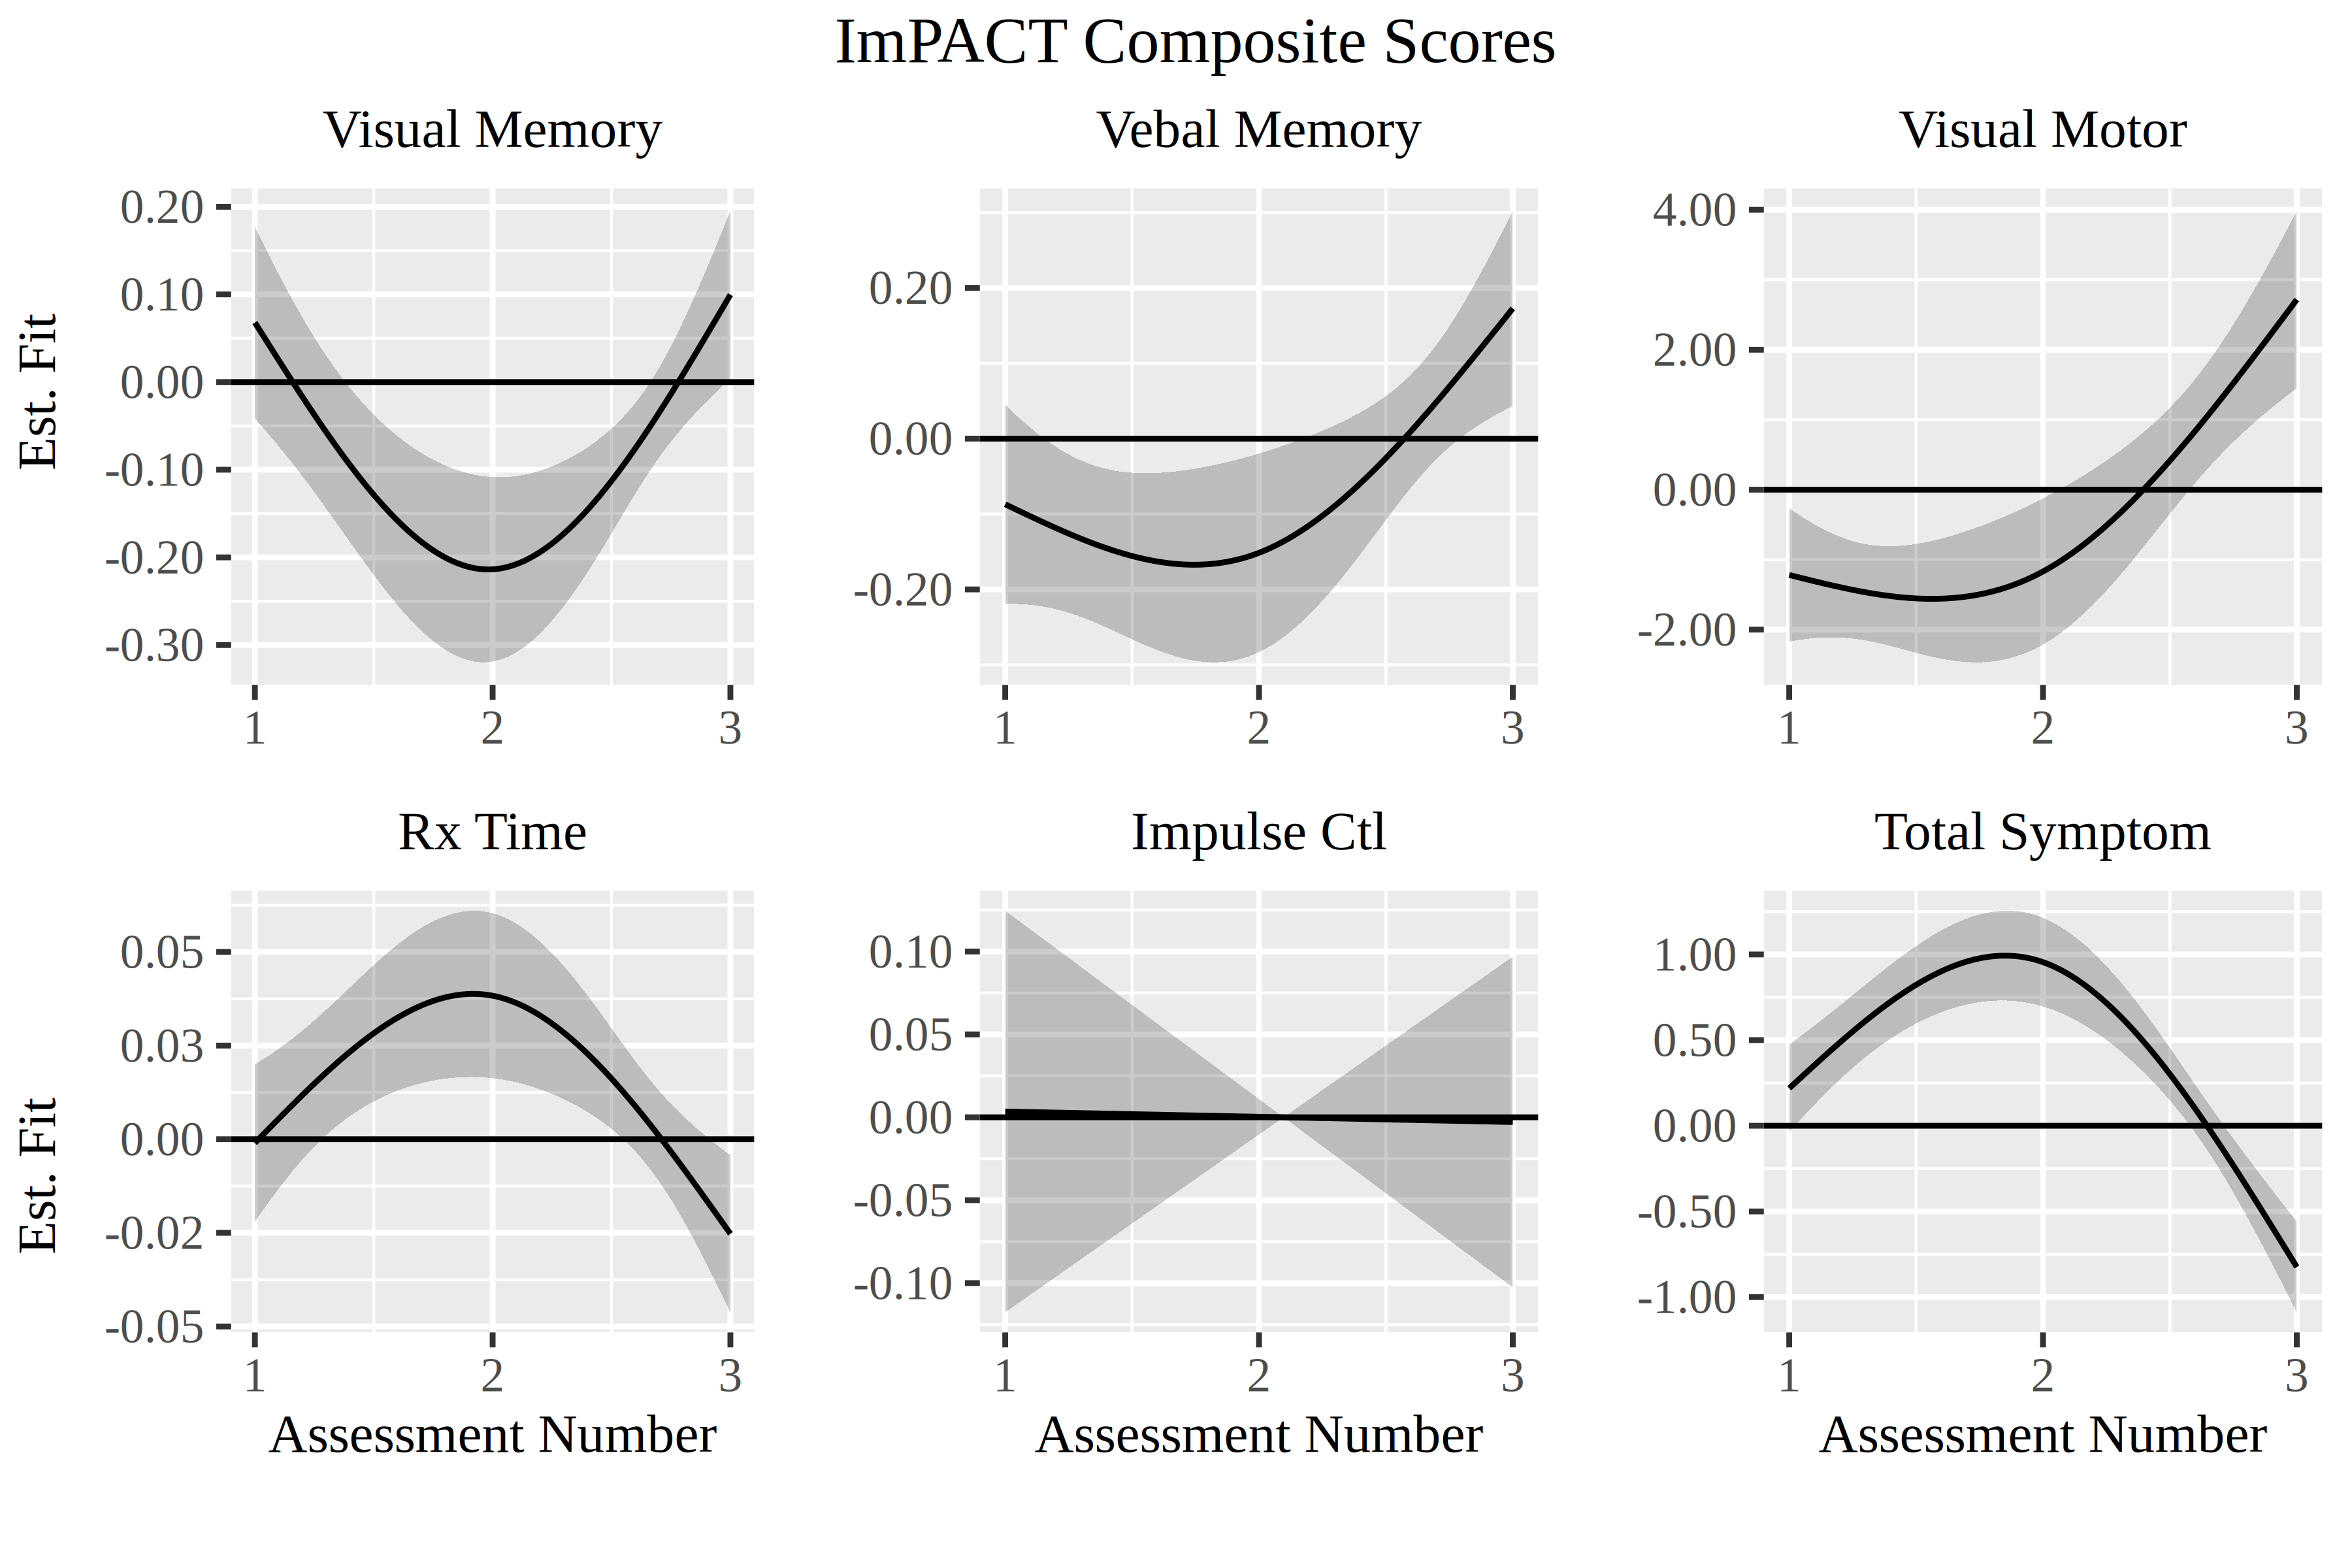
\includegraphics{fig_impact_gam.png}}
	\caption{GAM smooths for ImPACT composite and total symptom scores. Assessments where the confidence interval does not include 0 indicate significant changes. Visual memory, reaction time, and total symptoms showed worsening and then recovery (U-shapes) while verbal memory and visual motor scores were better at assessment 3. Impulse control did not change across assessments. Assessment number 1=Base, 2=Post, 3=RTP. Rx Time = reaction time, Impulse Ctl = impulse control.}
	\label{fig:imp-gam}
\end{figure}

All models except for impulse control detected a significant interaction between ImPACT metric and assessment. Visual memory, reaction time, and total symptoms had patterns consistent with concussion-related deficits at Post and subsequent recovery at RTP (visual memory: $F_{(1.94, 1.99)}$ = 8.59, \textit{p} $<$ .001; reaction time: $F_{(1.91, 1.99)}$ = 6.18, \textit{p} $<$ .01; total symptoms: $F_{(1.98, 1.99)}$ = 28.74, \textit{p} $<$ .0001), where we note that total symptoms at RTP were much lower than at Base (Figure \ref{fig:imp-gam}, bottom right). Conversely, while verbal memory and visual motor tests indicate significant non-flatness (verbal memory: $F_{(1.82, 1.96)}$ = 4.34, \textit{p} = .028; visual motor: $F_{(1.86, 1.97)}$ = 8.19, \textit{p} $<$ .001), their values did not differ between Base and Post while RTP was significantly better. This pattern possibly reflects a lack of sensitivity at Base and/or practice effects. Finally, impulse control was unchanged (i.e. flat) as a function of assessment ($F_{(1.0, 1)}$ = .003, \textit{p} = .95).


\subsection{DWI Tracts}
\label{ssec:res-dwi-tract}
Tract results.

% TODO: LDI, LGIO GAMs

\subsection{DWI Tracts Interactions - ImPACT}
\label{ssec:res-dwi-imp}
Description of DWI - ImPACT interaction.

% TODO: Motivate select tracts
% TODO: LGI_intx, LGIO_intx GAMs tracts - vis_mem?

\subsection{DWI Tracts Interactions - Time}
\label{ssec:res-dwi-time}
Description of DWI-time interaction.

% TODO: DI_time GAM results - rSLF?


\section{Discussion}
\label{sec:disc}
Discussion.

% TODO: Summary/recap
% TODO: Interpret main findings
% TODO: Advocate HGAMs for mTBI research


% acknowledgment page
\section*{Acknowledgments}
\label{sec:ack}
People. Grant.

% TODO: ariana for consulting


% write bibliography
\pagebreak
\printbibliography
\pagebreak


% make supplemental
\section{Supplemental Materials}
\label{sec:supp-materials}
\beginsupplement
Supplemental Materials.



\subsection{Tables}
\label{ssec:supp-tables}
Supplemental Tables.


\subsection{Figures}
\label{ssec:supp-figures}
Supplemental Figures.


\end{document}